\subsection{Electroweak Interactions}
\label{sec:Intro_Electroweak}

All electrically charged particles participate in electromagnetic interactions. The theory of electromagnetic interactions is called quantum electrodynamics (QED). All electromagnetic interactions are mediated by a photon, a spin-one electrically neutral massless particle, and can be reduced to one elementary process (Fig.~\ref{fig:feynmEM}, left). This process represents a charged fermion radiating or absorbing a photon. Such elementary process itself is forbidden by the energy conservation law but this element is a base of an actual process. For example, the Bhabha scattering, $e^+e^- \rightarrow e^+e^-$, occures through $e^+e^-$ annihilation with further production of a new $e^+e^-$ pair (Fig.~\ref{fig:feynmEM}, middle) or through exchange of a photon between the positron and the electron (Fig.~\ref{fig:feynmEM}, right). Both cases involve nothing except the electromagnetic elementary process (Fig.~\ref{fig:feynmEM}, left). Such graphical representations of the particle physics processes are called Feynman diagrams.\\ 

\begin{figure}[htb]
  \begin{center}
    {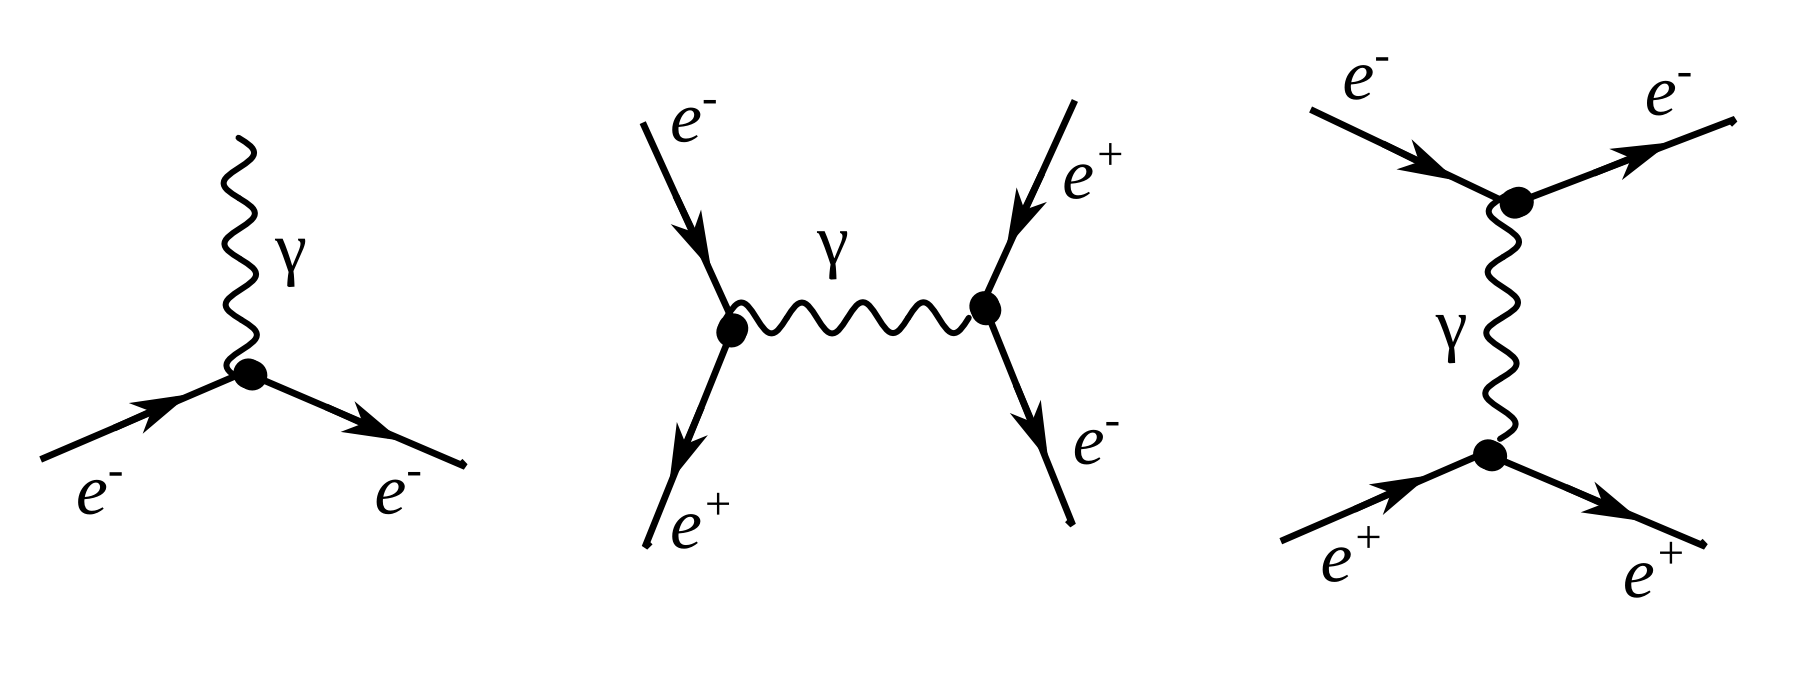
\includegraphics[width=0.90\textwidth]{../figs/Intro/feynmEM.png}}
    \caption{Electromagnetic interactions. Left: a photon radiation off a charged fermion, middle and right: Bhabha scattering. }
    \label{fig:feynmEM}
  \end{center}
\end{figure}

\begin{figure}[htb]
  \begin{center}
    {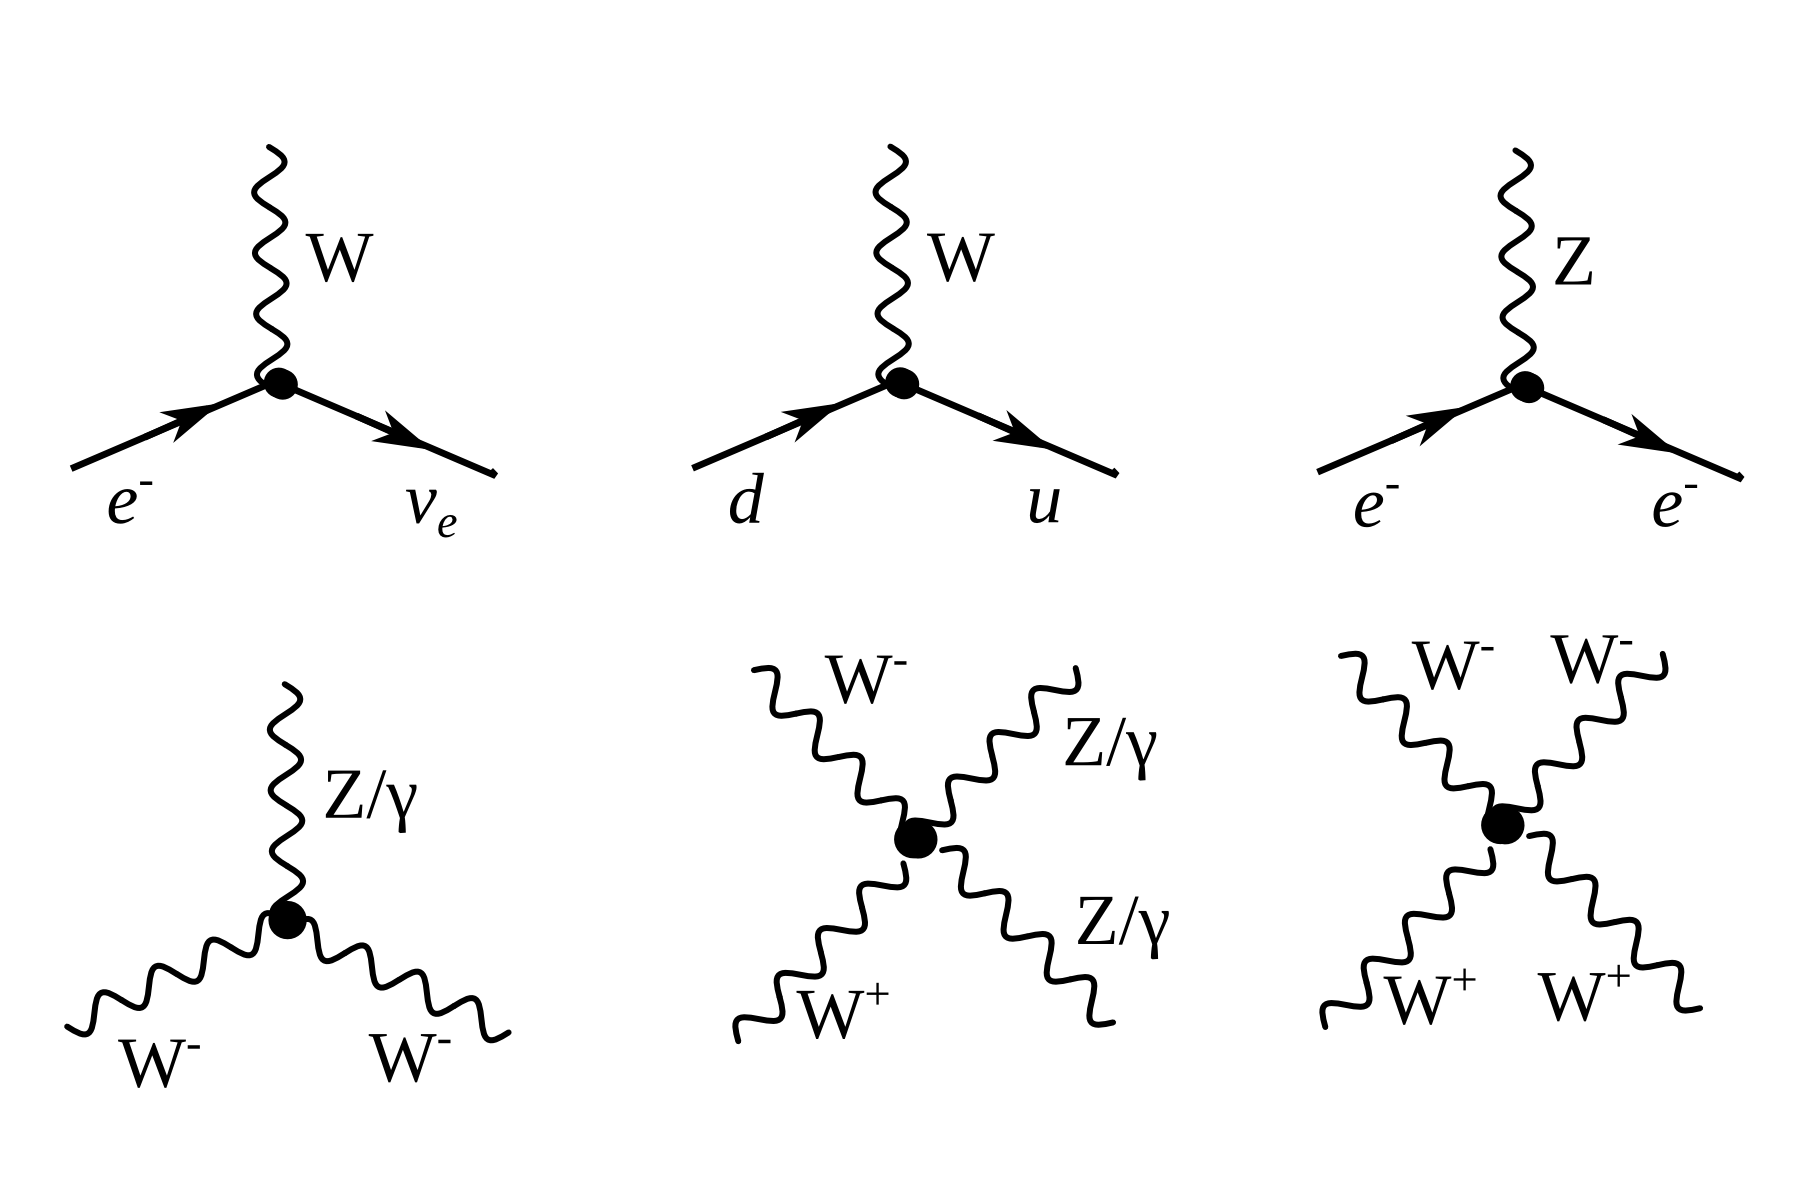
\includegraphics[width=0.90\textwidth]{../figs/Intro/feynmW.png}}
    \caption{Weak elementary processes and gauge couplings. Top left: a quark with charge Q=$+$2/3 enters, emits a $W$ boson, and a quark with charge Q=$-$1/3 escapes. Top middle: a charged lepton enters, emits a $W$ boson, and a neutrino or antineutrino escapes conserving a lepton flavor number. Top right: a fermion enters, emits a $Z$ boson and escapes. Bottom left: TGC couplings $WW\gamma$ and $WWZ$. Bottom middle: QGC couplings $WW\gamma\gamma$, $WWZ\gamma$ and $WWZZ$. Bottom right: QGC coupling $WWWW$.}
    \label{fig:feynmW}
  \end{center}
\end{figure}

As for the weak interactions, there are two kinds of them: neutral (mediated by a $Z$ boson) and charged (mediated by a $W^\pm$ boson). Elementary processes with $W$ and $Z$ bosons are shown in Fig.~\ref{fig:feynmW}. Because the electric charge must be conserved at any vertex, a particle radiating or absorbing a $W$ boson converts to a different particle. Thus, a charged lepton converts to a neutrino (or vice versa) as shown in Fig.~\ref{fig:feynmW}, top middle. Each lepton carries a lepton flavor number (Tab.~\ref{tab:LeptonFlavorNumber}). Lepton flavor is conserved in any interaction, thus an electron radiating a $W$ boson  always converts to an electron neutrino, a muon converts to a muon neutrino etc.\\

\begin{table}[h]
  \begin{center}
  \caption{ Lepton Flavor Number}
  \vspace{5 mm}
  \begin{tabular}{|c|c|c|c|}
     \hline
     particles & $L_e$ & $L_{\mu}$ & $L_{\tau}$ \\ \hline
     $e^-,\nu_e$ &  +1  &  0  &  0  \\ \hline 
     $e^+, \bar{\nu_e}$ &  -1  &  0  &  0  \\ \hline 
     $\mu^-,\nu_{\mu}$ &  0  &  +1  &  0  \\ \hline 
     $\mu^+, \bar{\nu_{\mu}}$ &  0  &  -1  &  0  \\ \hline 
     $\tau^-,\nu_{\tau}$ &  0  &  0  &  +1  \\ \hline 
     $\tau^+, \bar{\nu_{\tau}}$ &  0  &  0  &  -1  \\ \hline 
  \end{tabular}
  \label{tab:LeptonFlavorNumber}
  \end{center}
\end{table}

From top left diagram in Fig.~\ref{fig:feynmW} we see that if a quark with Q=$+$2/3 enters, then a quark with Q=$-$1/3 escapes and, therefore, the flavor of the quark is changed. The charged weak interaction is the only interaction which changes a quark flavor. The probability of each of three quarks with Q=$-$1/3 to be born is determined by the Cabibbo-Kobayashi-Maskawa matrix which relates mass eigenstates $d$, $c$ and $b$ to weak eigenstates $d'$, $c'$ and $b'$ (Eq.~\ref{eq:CKM}). Absolute values of the matrix elements are all known (Eq.~\ref{eq:CKM_magn}) and are the highest for the quark of the same generation as an initial state quark. In the particular case shown in the top left diagram in Fig.~\ref{fig:feynmW}, $u$ is the initial state quark and $d$ has the highest probability to be produced after an interaction with a $W$ boson but $s$ and $b$ can also be produced if there is enough energy.\\

\begin{equation}\label{eq:CKM}
  \begin{pmatrix} d' \\ s' \\ b' \end{pmatrix}
     =
  \begin{pmatrix} 
     V_{ud} & V_{us} & V_{ub} \\
     V_{cd} & V_{cs} & V_{cb} \\
     V_{td} & V_{ts} & V_{tb} \\ 
  \end{pmatrix}
  \begin{pmatrix} d \\ s \\ b \end{pmatrix}
\end{equation}

\begin{equation}\label{eq:CKM_magn}
  \begin{pmatrix} 
     |V_{ud}| & |V_{us}| & |V_{ub}| \\
     |V_{cd}| & |V_{cs}| & |V_{cb}| \\
     |V_{td}| & |V_{ts}| & |V_{tb}| \\ 
  \end{pmatrix}
    =
  \begin{pmatrix} 
     0.97 & 0.23 & 0.00 \\
     0.23 & 0.97 & 0.04 \\
     0.01 & 0.04 & 1.00 \\ 
  \end{pmatrix}
\end{equation}

An elementary process of a neutral weak interaction is an emission a $Z$ boson off a fermion line (right top diagram in Fig.~\ref{fig:feynmW}). Diagrams with a $Z$ boson are very similar to ones with a photon except a photon can only be radiated off a charged particle but a $Z$ boson can also be radiated off a neutrino or antineutrino.\\

The bottom diagrams in Fig.~\ref{fig:feynmW} are gauge bosons coupling diagrams including self-coupling of a $W$ boson, its interaction with a $Z$ boson and its electromagnetic radiation of a photon. Charge-conserving TGC and quartic gauge couplings (QGC) containing two or four $W$ bosons are all possible in the SM: $WWZ$, $WW\gamma$, $WWZZ$, $WWZ\gamma$, $WW\gamma\gamma$, and $WWWW$.\\

\begin{figure}[htb]
  \begin{center}
    {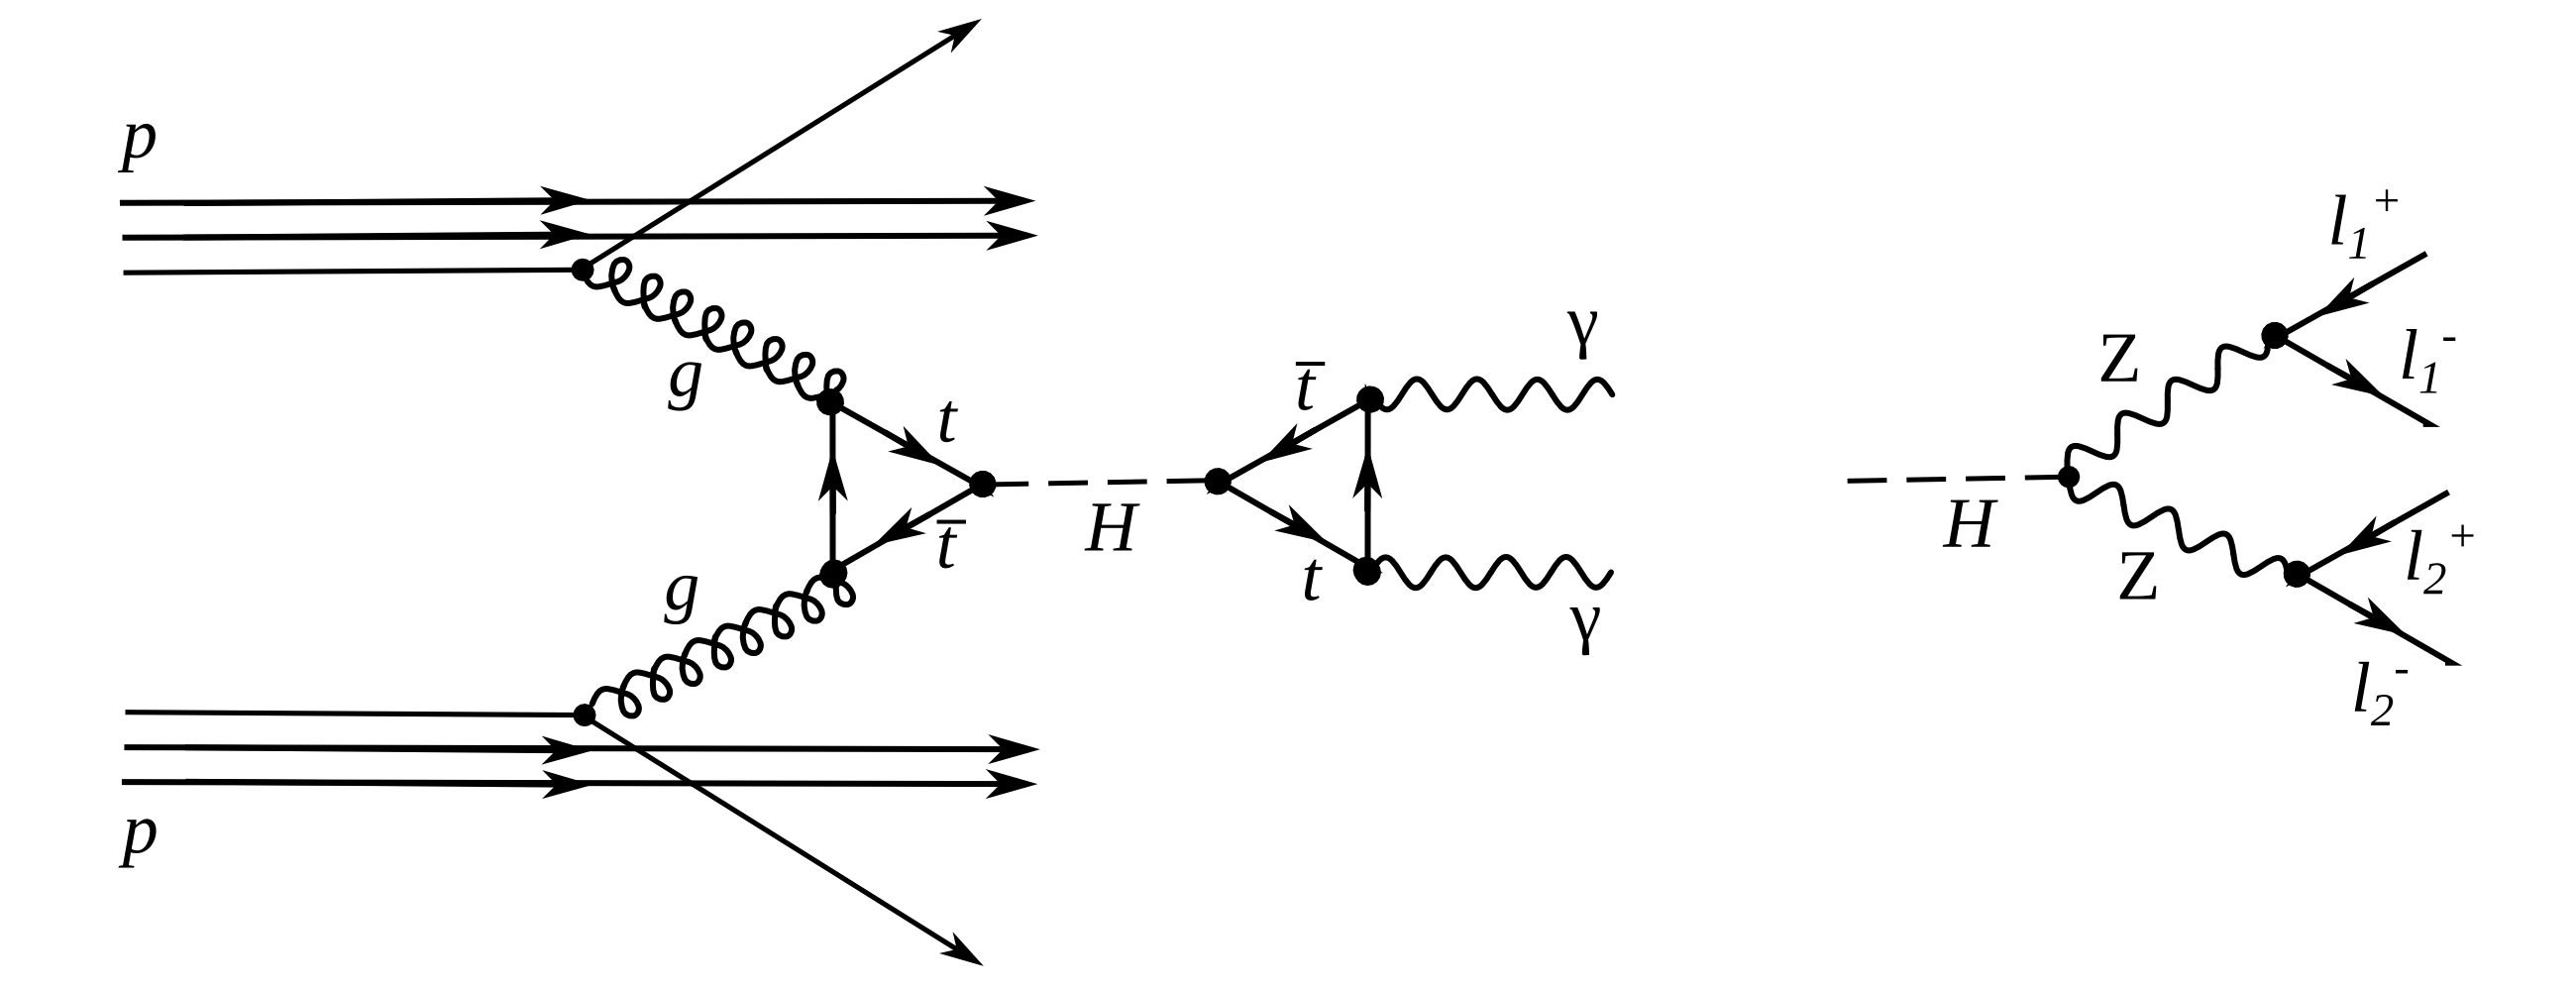
\includegraphics[width=0.95\textwidth]{../figs/Intro/FeynmanHiggs.png}}
    \caption{The Higgs boson production and decay. Left: $H\rightarrow\gamma\gamma$, right: $H\rightarrow ZZ \rightarrow 4l$.}
    \label{fig:higgsProduction}
  \end{center}
\end{figure}

Electromagnetic and weak interactions are unified by the electroweak Glashow-Weinberg-Salam (GWS) theory which is based on $SU(2) \times U(1)$ symmetry. $SU(2)$ is the symmetry of weak isospin which generates three bosons: $W^1$, $W^2$ and $W^3$. $U(1)$ is the symmetry of the weak hypercharge and generate one neutral boson $B$. $W^1$ and $W^2$ are mixed to create $W^+$ and $W^-$ mediators while $W^3$ and $B$ are mixed to create a $Z$ boson and a photon. Therefore, the GWS theory considers electromagnetic and weak forces as different manifestations of the electroweak force. The electroweak theory is discussed in greater details in Ch.~2.\\

However, weak interactions are mediated by heavy bosons ($M_W=80$ GeV, $M_Z=91$ GeV) while electromagnetic interactions are mediated by a massless photon, thus, the electroweak symmetry is broken. To explain this phenomenon, the Higgs mechanism was introduced. The mechanism predicted an existence of an additional boson: the Higgs boson. The Higgs boson was a missing piece of the SM for many years and was finally discovered in 2012 at LHC by ATLAS and CMS collaborations through the processes shown in Fig.~\ref{fig:higgsProduction}~\cite{ref_HiggsPaperCMS},~\cite{ref_HiggsPaperATLAS}.\\

The measurement in this dissertation is an electroweak measurement because the process involves a $W$ boson. It includes an interaction of a $W$ boson with leptons and quarks as well as the TGC $WW\gamma$. Thus, the measurement is a good test of the SM electroweak theory.\\ 


